\documentclass[conference]{IEEEtran}
\IEEEoverridecommandlockouts
\usepackage{cite}
\usepackage{amsmath,amssymb,amsfonts}
\usepackage{algorithmic}
\usepackage{flafter}
\usepackage{graphicx}
\usepackage{textcomp}
\usepackage{xcolor}
\graphicspath{ {imagenes/} }

\begin{document}

\title{Actividad G.5 \\ Terminal
}

\author{\IEEEauthorblockN{Ricardo David López Arellano}
\IEEEauthorblockA{\textit{Departamento de Ingeniería en Computación} \\
\textit{CUCEI}\\
Universidad de Guadalajara\\
ricardo.lopez1361@alumnos.udg.mx}
}
\onecolumn

\maketitle

\begin{abstract}
Se denomina terminal o consola (hardware) a un dispositivo electrónico o electromecánico que se utiliza para interactuar con un computador.
\end{abstract}

\begin{IEEEkeywords}
\begin{center}
Cursor, OS:gotoxy, OS:wherex, OS:wherey, count, cr, dup, over, getch, OS:key, 
\end{center}
\end{IEEEkeywords}

\section{Originalidad}
Me comprometo a producir trabajo académico íntegro, lo que significa un trabajo que se adhiere a los estándares intelectuales y académicos de atribución exacta de las fuentes, uso y recolección de datos apropiados, y transparencia en el reconocimiento de las contribuciones de las ideas, descubrimientos, interpretaciones y conclusiones de otros.
Acepto que la trampa en los exámenes, el plagio o la fraudulenta representación de las ideas o lenguaje de otros como propio, la falsificación de datos o cualquier otra instancia de deshonestidad académica, violan los estándares de LA MATERIA, así como los estándares del mundo en general en el campo del conocimiento y las relaciones.

\section{Introducción}
\begin{center}
Una terminal es un programa cuyo objetivo principal es leer comandos y ejecutar otros programas. Las principales ventajas de la terminal son su alta relación acción-tecla, su soporte para la automatización de tareas repetitivas, y que puede utilizarse para acceder a otras máquinas en una red.

\end{center}

\section{Objetivos de la actividad}
\begin{center}
 • Manipular la terminal mediante el uso de palabras orientadas a la misma.
\end{center}

\section{Metodología}
OS:gotoxy: es una palabra que mueve el cursor a la posición requerida (coordenadas x, y) pasadas a través de la pila de datos. \\
\\OS:wherex: regresa la coordenada 'x' de la posición del cursor en la pila de datos. \\
\\OS:wherey: regresa la coordenada 'y' de la posición actual del cursor en la pila de datos. \\
\\Count: palabra que regresa el número de símbolos que contiene el texto que se encuentra en la celda superior de la pila de direcciones. Además, es importante señalar que dicha cuenta no incluye el símbolo de terminación nulo. \\
\\cr: palabra que imprime un salto de línea en la terminal. \\
\\dup: palabra que crea una copia del texto que se encuentra en la celda superior en la pila de direcciones. \\
\\over: palabra que duplica la segunda celda en la pila de direcciones. \\
\\OS:getch: palabra que lee un byte procedente de teclado y lo guarda en la pila de datos. \\
\\OS:key: palabra que lee un símbolo (de 1 o más bytes) procedente del teclado y lo guarda en la pila de datos. \\ 

\section{Contenido}
\subsection{Estructuras:}
Entrada de usuario: \\
El usuario puede interactuar con un programa mediante diversos dispositivos, entre los cuales se encuentra el teclado, el cual está inspirado en el teclado de las máquinas de escribir, presentando diferentes disposiciones de las teclas. Por otro lado, en esta sección se abordarán las instrucciones que permiten leer las teclas presionadas por el usuario. \\
\\Texto: \\
Un texto o cadena de texto es una espacio en memoria que contiene una secuencia de símbolos (caracteres) y tiene una longitud arbitraria, terminando en un símbolo nulo equivalente a 00 hexadecimal. Además, es importante señalar que los símbolos en dicho texto pueden tener una longitud igual o mayor a un byte. Por otro lado, para introducir un texto se deben poner los símbolos entre comillas dobles, por ejemplo, "hola mundo", donde dicha cadena de texto se guardará en la pila de apuntadores. Además, en el caso de los símbolos se escriben entre comillas simples, por ejemplo, 'a', y dichos símbolos se guardan en la pila de datos. \\
\\Cursor: \\
Se denomina terminal o consola (hadware) a un dispositivo electrónico o electromecánico que se utiliza para interactuar con un computador. Generalmente la terminal soporto códigos de escape (ESC), los cuales permiten cambiar colores, mover el cursor, entre otros. Además, dichos códigos se pueden utilizar mediante un texto enviado a la terminal que contiene "ESC[7m". donde después del corchete cuadrado se debe especificar el código a utilizar. Por otro lado, en esta sección se abordarán las instrucciones que permiten mover el cursor en la terminal.

\section{Resultados}
\begin{enumerate}
\item  EJERCICIO 1:\\
	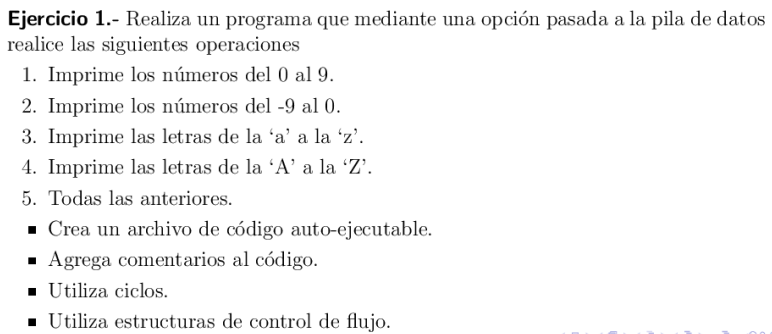
\includegraphics{e1} \\
	\begin{center}
	\textbf{Respuesta: } 5 \\ if dup 1 = \\  0 . \\  0 \\  dup \\ while 9 < \\ 1 + \\ dup  . \\ dup \\ elif dup 2 = \\ -9 \\  while dup \\ dup S. \\ ++ \\ 0 . \\ elif dup 3 = \\ for 97 upto 122 \\ dup emit \\ elif dup 4 = \\ 65 \\ repeat \\ dup emit \\  ++ \\ dup \\ until 91 = end \\ elif dup 5 = \\ 0 . \\ 0 \\  dup \\ while 9 < \\ 1 + \\ dup . \\ dup \\ cr \\ -9 \\  while dup \\ dup S. \\ ++ \\ 0 . \\ cr \\ for 97 upto 122 \\ dup emit \\ cr \\ 65 \\  repeat \\  dup emit \\  ++ \\  dup \\  until 91 = \\ end \\  cr \\
	\end{center}
	
\item  EJERCICIO 2:\\
	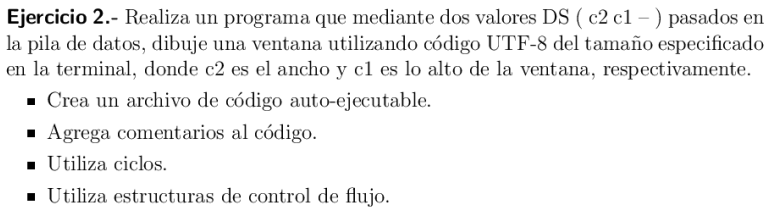
\includegraphics{e2} \\
	\begin{center}
	\textbf{Respuesta: } 10 //ALTO \\ 80  //ANCHO \\ 2 - \\ swap \\ 2 - \\ swap \\ DS. \\ "-" . \\ //hacer la esquina superior izquierda \\ dup \\ while dup 0 > //condicion para hacer la linea horziontal \\ "-" . \\  1 - \\ swap \\ "-" . //hacer la esquina superior derecha \\ cr \\ swap \\ drop \\ swap \\ dup \\ swap \\ rot \\ swap \\ while dup 0 > //hacer la esquina superior vertical \\ "l". \\   swap \\   dup \\   while dup 0 > \\ " ". //agregar los espacios para que quede rectangular \\ 1 - \\   drop \\   swap \\   1 - \\   "l" . //fin de cuadro (linea vertical) \\   cr \\ drop \\ "-" . //hacer la esquina \\ inferior izquierda \\ dup \\ while dup 0 > \\  "-" . \\  1 - \\ swap \\ "-". //hacer la esquina inferior \\ derecha \\ swap \\ drop \\ cr \\
	\end{center}

\end{enumerate}

\section{Resultados (diagramas de flujo)}
\begin{enumerate}
  	\item EJERCICIO 1 y 2:\\
  	\begin{center}
	Los diagramas se mostrarán en formato .png fuera del PDF. Ya que son demasiado grandes para ingresarlos en un hoja.
	\end{center}

\end{enumerate}

\section{Conclusiones}  
En conclusión de esta tarea puedo decir que estos ejercicio fáciles aunque ya va subiendo su complejidad no estan tan complicados ya que con conocimientos que ya tenia pude realizarlos. Pero es bueno aprender un lenguaje nuevo ya que yo ni si quiera había utilizado Linux ni mucho menos Latex, así que es una buena experiencia.

\section*{Agradecimientos}
Quiero hacer agradecimiento a mi profesor por explicarme cuando tenia dudas sobre cómo hacer los ejercicios, a mis compañeros porque varias veces me brindaron ayuda cuando tenia problemas y a mis padres en apoyarme cuando los necesito.

\begin{thebibliography}{00}
\bibitem{Alvarez2022} Becerra Alvarez, E. C. (2022, 4 octubre). ForEmb. https://drive.google.com/file/d/1Vs3F8gG-VkG6kugb4hsUSh2wFX9tYU0R/view
\end{thebibliography}

\end{document}
